% -*- eval: (load-file "./autoloader.el")  -*-

\documentclass[25pt, a0paper, portrait]{tikzposter}
\title{\parbox{\linewidth}{\centering Transparently Using Non-Volatile Memory with Taenite, A Rust Transactional NVM Library}}
\author{Louis Boulanger, Yves Denneulin, Frédéric Wagner}
\institute{Univ. Grenoble Alpes, CNRS, Inria, Grenoble INP, LIG}

\usetikzlibrary{arrows, arrows.meta, decorations.pathreplacing, patterns.meta}
\usepackage{lmodern}
\usepackage{minted}

% Arial-like font, Helvetica
\usepackage{helvet}
\renewcommand\familydefault{\sfdefault}


% \Huge isn't enough. First argument to \fontsize is the size, second is spacing (should be 1.2x font size)
\newcommand*{\HUGE}{\fontsize{80}{96}\selectfont}

% Color palette and style
\definecolorstyle{LIGStyle}{
  \definecolor{LIGBlue}{cmyk}{0.85,0.6,0.12,0}
  \definecolor{LIGLightBlue}{cmyk}{0.82,0.46,0,0}
  \definecolor{LIGGray}{cmyk}{0.64,0.54,0.52,0.52}
}{
  \colorlet{backgroundcolor}{white}
  \colorlet{framecolor}{white}
  \colorlet{titlefgcolor}{white}
  \colorlet{titlebgcolor}{LIGBlue}
  \colorlet{blocktitlebgcolor}{white}
  \colorlet{blocktitlefgcolor}{LIGBlue}
  \colorlet{blockbodybgcolor}{white}
  \colorlet{blockbodyfgcolor}{black}
}
\usecolorstyle{LIGStyle}

% Title style
\definetitlestyle{LIGTitle}{
  width=0.9\paperwidth, roundedcorners=0, 
}{
  \begin{scope}[line width=\titlelinewidth, rounded corners=\titleroundedcorners]
  \end{scope}
}

% Title format
\settitle{
  \vspace{-8mm}
  \centering\color{titlefgcolor}{\textbf{\HUGE \sffamily \@title}}
  
  {
    \vspace{30mm}
    \color{blockbodyfgcolor}{\LARGE \sffamily \@author \par}
    \vspace{1em}
    \color{blockbodyfgcolor}{\Large \sffamily \@institute \par}
  }
}

% Block style
\defineblockstyle{LIGBlock}{
  bodywidthscale=1
}{
  \ifBlockHasTitle
  \draw [line width=1mm] (blockbody.north west) -- (blockbody.north east);
  \fi
}

\usetitlestyle{LIGTitle}
\useblockstyle{LIGBlock}

\begin{document}
% Add LIG template png as background image
\node[above right,opacity=1,inner sep=0pt,outer sep=0pt] at (bottomleft) {\includegraphics[width=\paperwidth,height=\paperheight]{template}};

\maketitle

% Amazingly, tikzposter doesn't define "topleft" and "bottomright".
\coordinate (topleft)     at (topright -| bottomleft);
\coordinate (bottomright) at (topright |- bottomleft);

% Bar to separate authors from contents.
% Default tikz units are in cm, and A0 is 84.1cmx118.9cm. (0, 0) is the center of the page.
\draw[black, thick, line width=2mm, color=LIGBlue] (-42.05, 43) -- (42.05, 43);

% Linked list node
\newcommand\LLNode[4]{
  \node[draw, line width=1mm, minimum height = 15mm, minimum width = 15mm, black, text = black, fill = #4!25!white] at (#1) (#2block) {#3};
  \node[draw, line width=1mm, minimum height = 5mm, minimum width = 15mm, anchor = north, black, fill = #4!15!white] at ([yshift=\pgflinewidth]#2block.south) (#2ptr) {};
}
\newcommand\LLNodeH[4]{
  \node[draw, line width=1mm, minimum height = 15mm, minimum width = 15mm, black, text = black, fill = #4!25!white] at (#1) (#2block) {#3};
  \node[draw, line width=1mm, minimum height = 15mm, anchor = west, black, fill = #4!15!white] at ([xshift=-\pgflinewidth]#2block.east) (#2ptr) {};
}


\begin{columns}
  \column{0.5}
  \block{Why is NVRAM ``challenging'' to use?}{
    \begin{tikzfigure}[A memory hierarchy model including NVRAM\par]
      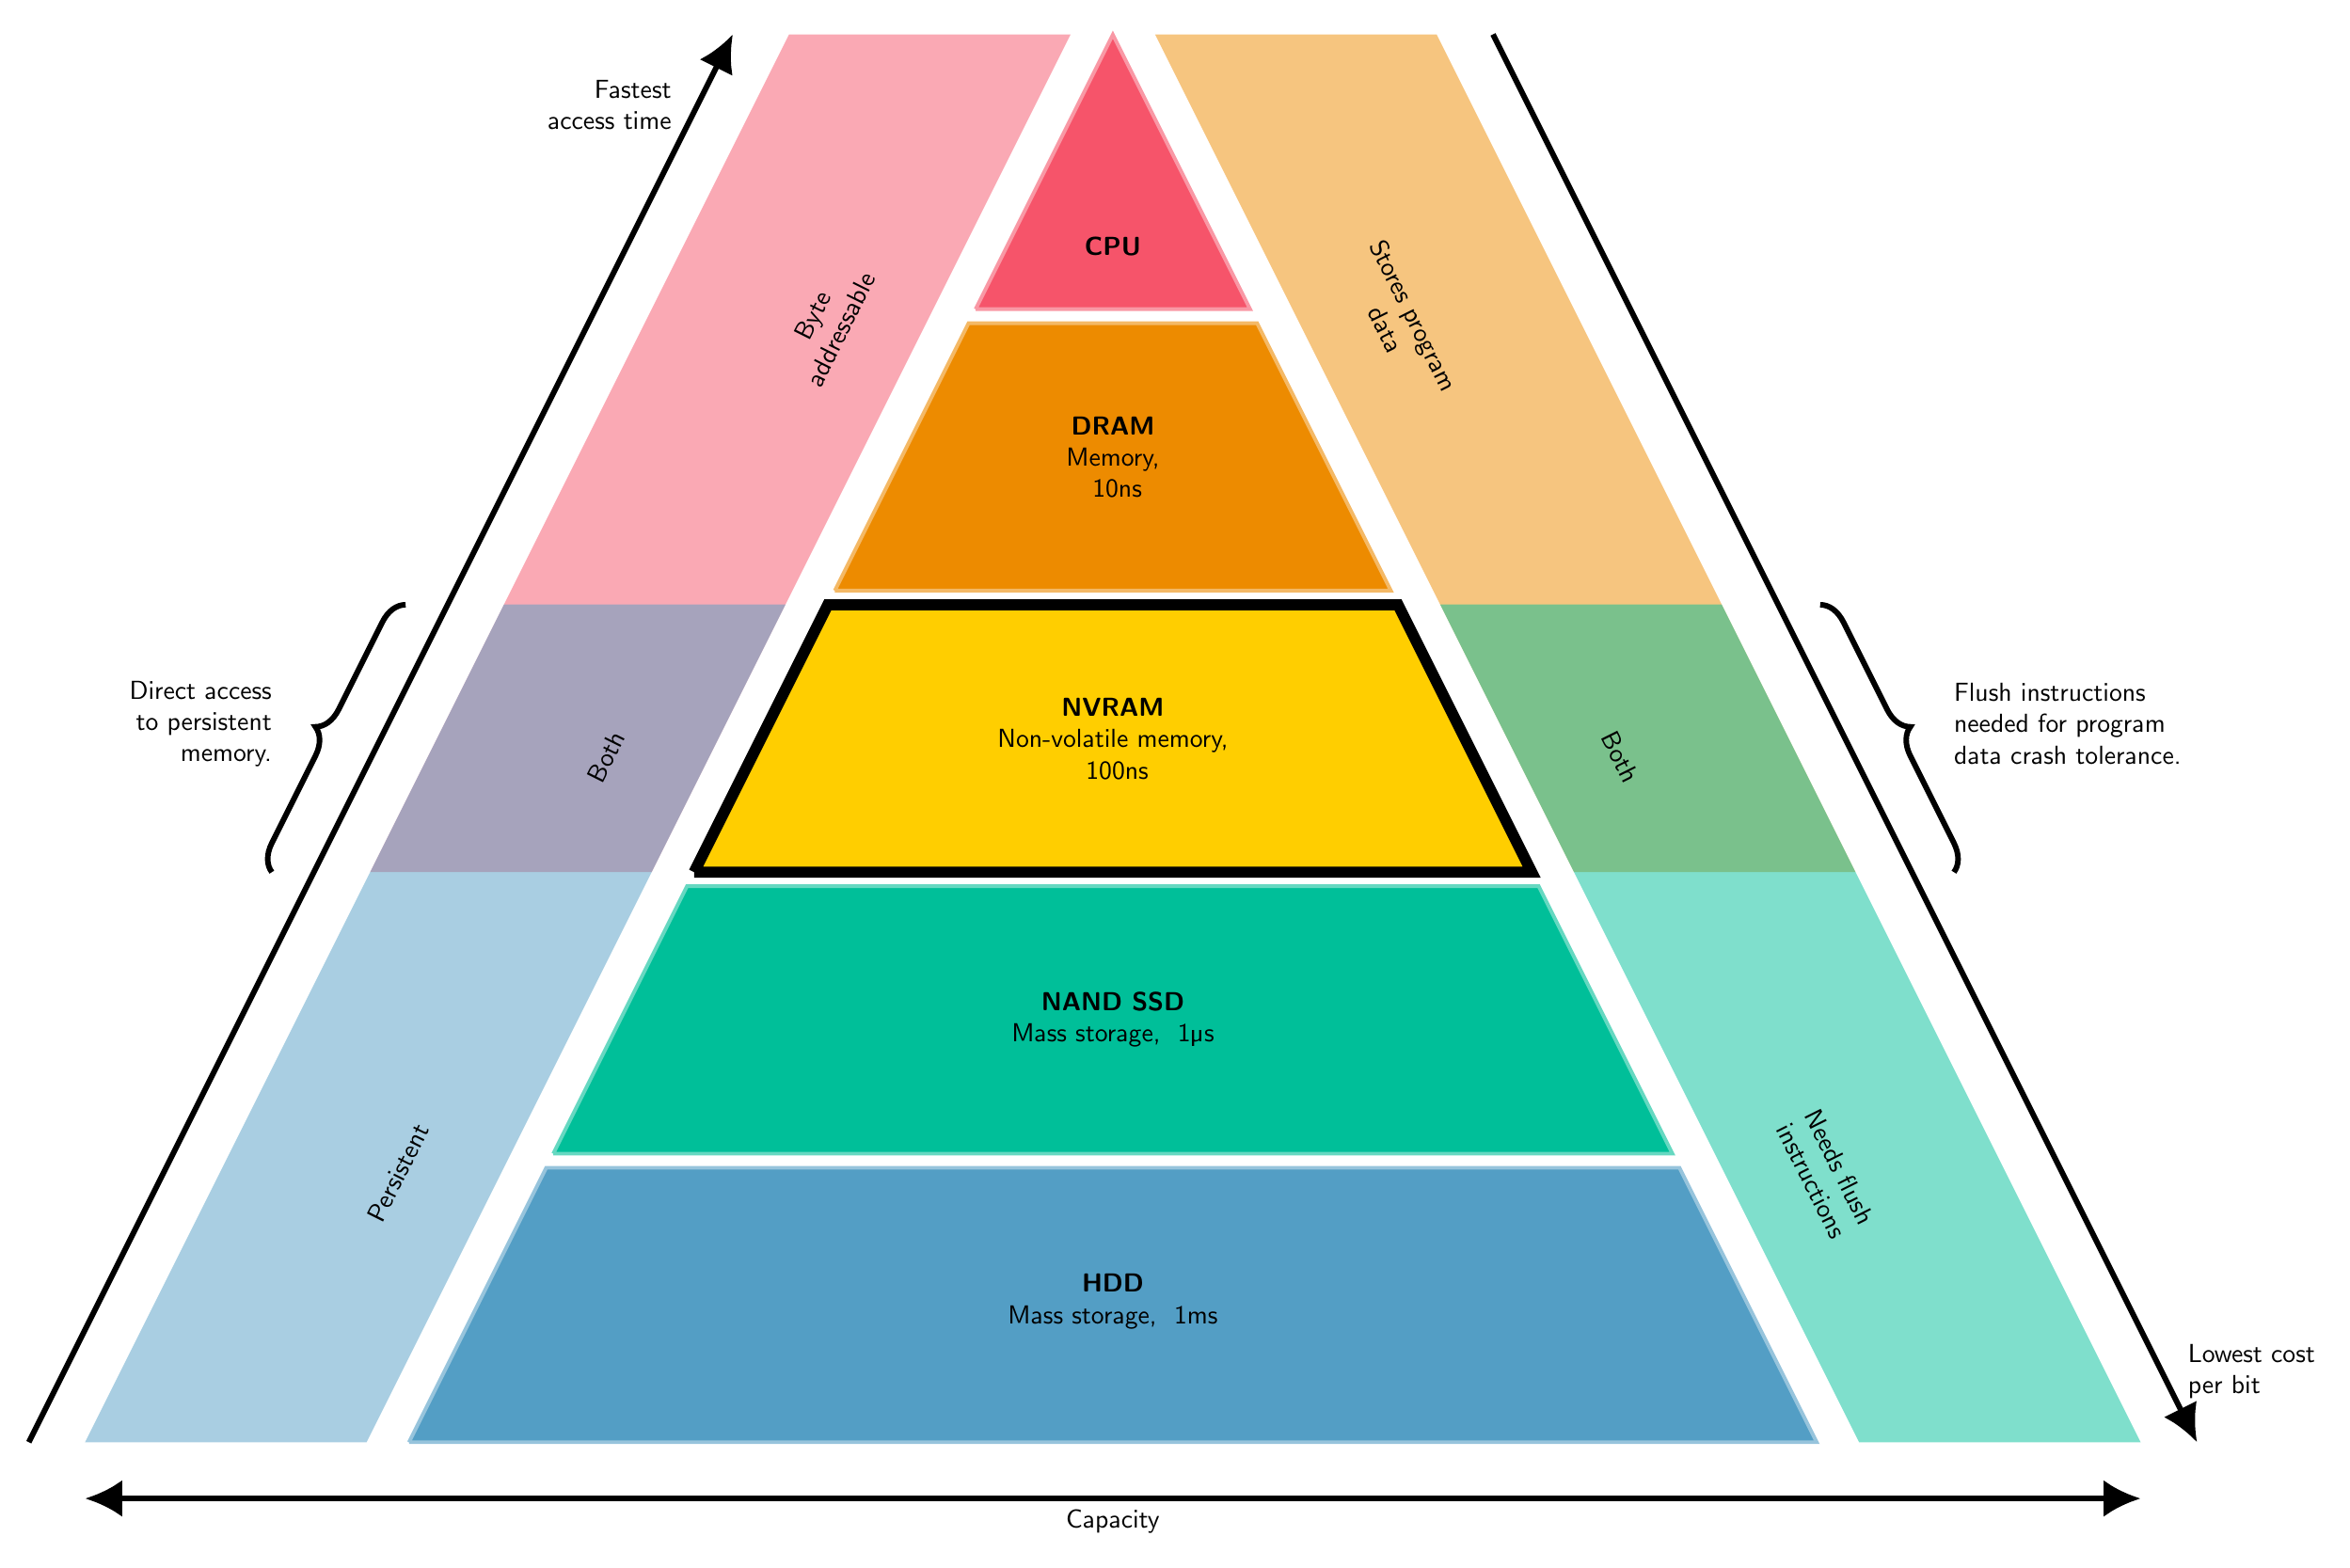
\begin{tikzpicture}[scale=1.9]
        \tikzstyle{every node}=[font=\normalsize]
        \definecolor{myblue}{RGB}{83,158,197}
        \definecolor{mylightblue}{RGB}{151,196,220}
        \definecolor{mygreen}{RGB}{0,191,153}
        \definecolor{mylightgreen}{RGB}{102,216,193}
        \definecolor{myyellow}{RGB}{255,206,0}
        \definecolor{mylightyellow}{RGB}{255,230,127}
        \definecolor{myorange}{RGB}{237,139,0}
        \definecolor{mylightorange}{RGB}{244,185,102}
        \definecolor{myred}{RGB}{246,84,106}
        \definecolor{mylightred}{RGB}{249,152,165}
        \node (a1) at (-5, 0) {};
        \node (a2) at (5, 0) {};
        \node (a3) at (-4.025, 1.95) {};
        \node (a4) at ( 4.025, 1.95) {};
        \draw[mylightblue, fill=myblue, line width=0.5mm] (a1.center) -- (a2.center) -- (a4.center) -- (a3.center) -- (a1.center);
        \node[align=center] (a5) at (0, 1) {\textbf{HDD}\\Mass storage, ~1ms};
        \node (b1) at (-3.975, 2.05) {};
        \node (b2) at ( 3.975, 2.05) {};
        \node (b3) at (-3.025, 3.95) {};
        \node (b4) at ( 3.025, 3.95) {};
        \draw[mylightgreen, fill=mygreen, line width=0.5mm] (b1.center) -- (b2.center) -- (b4.center) -- (b3.center) -- (b1.center);
        \node[align=center] (b5) at (0, 3) {\textbf{NAND SSD}\\Mass storage, ~1µs};
        \node (c1) at (-2.975, 4.05) {};
        \node (c2) at ( 2.975, 4.05) {};
        \node (c3) at (-2.025, 5.95) {};
        \node (c4) at ( 2.025, 5.95) {};
        \draw[black, fill=myyellow, line width=1.5mm] (c1.center) -- (c2.center) -- (c4.center) -- (c3.center) -- (c1.center);
        \node[align=center] (c5) at (0, 5) {\textbf{NVRAM}\\Non-volatile memory,\\~100ns};
        \node (d1) at (-1.975, 6.05) {};
        \node (d2) at ( 1.975, 6.05) {};
        \node (d3) at (-1.025, 7.95) {};
        \node (d4) at ( 1.025, 7.95) {};
        \draw[mylightorange, fill=myorange, line width=0.5mm] (d1.center) -- (d2.center) -- (d4.center) -- (d3.center) -- (d1.center);
        \node[align=center] (d5) at (0, 7) {\textbf{DRAM}\\Memory,\\~10ns};
        \node (e1) at (-0.975, 8.05) {};
        \node (e2) at ( 0.975, 8.05) {};
        \node (e3) at (0, 10) {};
        \draw[mylightred, fill=myred, line width=0.5mm] (e1.center) -- (e2.center) -- (e3.center) -- (e1.center);
        \node[align=center] (e4) at (0, 8.5) {\textbf{CPU}};
        \node (g1) at ([xshift = -0.3cm] e3.center) {};
        \node (g2) at ([xshift = -2.3cm] e3.center) {};
        \node (g3) at ([xshift = -2.3cm] c1.center) {};
        \node (g4) at ([xshift = -0.3cm] c1.center) {};
        \draw[myred, fill=myred, fill opacity = 0.5, draw opacity = 0] (g1.center) -- (g2.center) -- (g3.center) -- (g4.center) -- (g1.center);
        \node (h1) at ([xshift = -0.3cm] c3.center) {};
        \node (h2) at ([xshift = -2.3cm] c3.center) {};
        \node (h3) at ([xshift = -2.3cm] a1.center) {};
        \node (h4) at ([xshift = -0.3cm] a1.center) {};
        \draw[myblue, fill=myblue, fill opacity = 0.5, draw opacity = 0] (h1.center) -- (h2.center) -- (h3.center) -- (h4.center) -- (h1.center);

        \draw[draw opacity = 0] ([xshift = -0.3] d1.center) -- ([xshift = -0.3] e3.center) node [midway, above, sloped, anchor = south, xshift = -1cm, yshift = 1.25cm, text width = 3cm, align = center] {Byte\\addressable};
        \draw[draw opacity = 0] ([xshift = -0.3] a1.center) -- ([xshift = -0.3] b3.center) node [midway, above, sloped, anchor = south, xshift = -1cm, yshift = 1.5cm, text width = 3cm, align = center] {Persistent};
        \draw[draw opacity = 0] ([xshift = -0.3] c1.center) -- ([xshift = -0.3] c3.center) node [midway, above, sloped, anchor = south, xshift = -1.15cm, yshift = 1.5cm, text width = 3cm, align = center] {Both};

        \draw[decorate, decoration = {brace, amplitude = 10pt}, black, line width = 0.75mm] ([xshift = -3cm] c1.center) -- ([xshift = -3cm] c3.center) node [midway, xshift = -0.75cm, yshift=0.2cm, anchor = east, align = right] {Direct access\\to persistent\\memory.};

        
        \node (i1) at ([xshift = 0.3cm] e3.center) {};
        \node (i2) at ([xshift = 2.3cm] e3.center) {};
        \node (i3) at ([xshift = 2.3cm] c2.center) {};
        \node (i4) at ([xshift = 0.3cm] c2.center) {};
        \draw[myorange, fill=myorange, fill opacity = 0.5, draw opacity = 0] (i1.center) -- (i2.center) -- (i3.center) -- (i4.center) -- (i1.center);
        \node (j1) at ([xshift = 0.3cm] c4.center) {};
        \node (j2) at ([xshift = 2.3cm] c4.center) {};
        \node (j3) at ([xshift = 2.3cm] a2.center) {};
        \node (j4) at ([xshift = 0.3cm] a2.center) {};
        \draw[mygreen, fill=mygreen, fill opacity = 0.5, draw opacity = 0] (j1.center) -- (j2.center) -- (j3.center) -- (j4.center) -- (j1.center);

        \draw[draw opacity = 0] ([xshift = 0.3] d2.center) -- ([xshift = 0.3] e3.center) node [midway, above, sloped, anchor = south, xshift = 1cm, yshift = 1.25cm, text width = 7cm, align = center] {Stores program\\data};
        \draw[draw opacity = 0] ([xshift = 0.3] a2.center) -- ([xshift = 0.3] b4.center) node [midway, above, sloped, anchor = south, xshift = 1cm, yshift = 1.25cm, text width = 6cm, align = center] {Needs flush\\instructions};
        \draw[draw opacity = 0] ([xshift = 0.3] c2.center) -- ([xshift = 0.3] c4.center) node [midway, above, sloped, anchor = south, xshift = 1.15cm, yshift = 1.5cm, text width = 3cm, align = center] {Both};

        \draw[decorate, decoration = {brace, amplitude = 10pt, mirror}, black, line width = 0.75mm] ([xshift = 3cm] c2.center) -- ([xshift = 3cm] c4.center) node [midway, xshift = 0.75cm, yshift=0.2cm, anchor = west, align = left] {Flush instructions\\needed for program\\data crash tolerance.};

        
        \path [-{Latex[length=5mm,width=5mm]}, line width=0.75mm] ([xshift=-0.4cm]h3.center) edge node[pos = 0.95, anchor = east, align = right, xshift=-0.2cm] {Fastest\\access time} ([xshift=-0.4cm]g2.center);
        \path [-{Latex[length=5mm,width=5mm]}, line width=0.75mm] ([xshift=0.4cm]i2.center) edge node[pos = 0.95, anchor = west, align = left, xshift=0.2cm] {Lowest cost\\per bit} ([xshift=0.4cm]j3.center);
        \path [{Latex[length=5mm,width=5mm]}-{Latex[length=5mm,width=5mm]}, line width=0.75mm] ([yshift=-0.4cm]h3.center) edge node[sloped, anchor=center, below] {Capacity} ([yshift=-0.4cm]j3.center);
        

      \end{tikzpicture}
    \end{tikzfigure}
  }

  \block{Immutable structures as an alternative to journals}{
    \centering Example: a Linked List ``ACD'' $\rightarrow$ ``ABCD''.
    \vspace{2em}

    \begin{minipage}{0.48\linewidth}
      \centering \textbf{Transaction journals}
      \begin{tikzfigure}[An example of a linked list to which a node is added after the head. The persistency is secured through a transactionnal journal.\par]        
        \begin{tikzpicture}
          \LLNode{0,0}{b0}{A}{black!50!green};
          \LLNode{0,-3}{a1}{B}{black!50!green};
          \LLNode{0,-6}{b1}{C}{red};
          \LLNode{0,-9}{b2}{D}{red};

          \node[draw, line width = 1mm, minimum width = 5cm] at ([xshift = 8cm]b0block.center) (j0) {Journal};
          \node[draw, line width = 1mm, minimum width = 5cm, anchor = north] at ([yshift = \pgflinewidth]j0.south) (j1) { \dots };
          \node[draw, line width = 1mm, minimum width = 5cm, anchor = north, minimum height = 3cm] at ([yshift = \pgflinewidth]j1.south) (j5) {  };
          \node[draw, line width = 1mm, minimum width = 5cm, anchor = north, minimum height = 3cm] at ([yshift = \pgflinewidth]j5.south) (j2) {  };
          \node[draw, line width = 1mm, minimum width = 5cm, anchor = north] at ([yshift = \pgflinewidth]j2.south) (j4) { \dots };
          
          \LLNode{[yshift = 0.35cm]j2.center}{j3}{A}{red};
          
          \path[draw, -{Latex[length=5mm,width=5mm]}, line width=1mm] (b0ptr.center) -- (a1block.north);
          \path[draw, -{Latex[length=5mm,width=5mm]}, line width=1mm] (a1ptr.center) -- (b1block.north);
          \path[draw, -{Latex[length=5mm,width=5mm]}, line width=1mm] (b1ptr.center) -- (b2block.north);
          \path[draw, -{Latex[length=5mm,width=5mm]}, line width=1mm] (j3ptr.center) -| ([xshift = 3cm]b1block.east) -- (b1block.east);
          
          \path[draw, -{Rays}, line width=1mm] (b2ptr.center) -- ([yshift=-1cm]b2ptr.center);
          \path[draw, dashed, -{Latex[length=5mm,width=5mm]}, line width = 1mm] (j2.west) -- (b0block.east);
          \node[align = center] at (j5.center) {\small Allocation\\\small(16B)};
          \path[draw, dashed, -{Latex[length=5mm,width=5mm]}, line width = 1mm] (j5.west) -- (a1block.east);
          
        \end{tikzpicture}
      \end{tikzfigure}

    \end{minipage}
    \hfill
    \begin{minipage}{0.48\linewidth}
      \centering \textbf{Immutable data structures}
      \begin{tikzfigure}[The same operation, now with an immutable approach to the linked list (copy-on-write).\par]        
        \begin{tikzpicture}
          \LLNodeH{0,0}{b0}{A}{red};
          \LLNodeH{6,0}{b1}{C}{red};
          \LLNodeH{9,0}{b2}{D}{red};
          \LLNodeH{0,3}{a0}{A}{black!50!green};
          \LLNodeH{3,3}{a1}{B}{black!50!green};

          \node[anchor = east] at ([xshift=-0.5cm] b0block.west) {Original};
          \node[anchor = east] at ([xshift=-0.5cm] a0block.west) {New};
          
          \path[draw, -{Latex[length=5mm,width=5mm]}, line width=1mm] (b0ptr.center) -- (b1block.west);
          \path[draw, -{Latex[length=5mm,width=5mm]}, line width=1mm] (b1ptr.center) -- (b2block.west);
          \path[draw, -{Latex[length=5mm,width=5mm]}, line width=1mm] (a0ptr.center) -- (a1block.west);
          \path[draw, -{Latex[length=5mm,width=5mm]}, line width=1mm] (a1ptr.center) -| (b1block.north);
          \path[draw, -{Rays}, line width=1mm] (b2ptr.center) -- ([xshift=2cm]b2ptr.center);

          \path (0, -4.5);
          \path (0,  7.5);
        \end{tikzpicture}
      \end{tikzfigure}

    \end{minipage}
  }
  
  \block{Rust, a systems programming language}{
    \begin{minipage}{0.48\linewidth}
      \inputminted[autogobble]{rust}{showcase.rs}
    \end{minipage}
    \hfill
    \begin{minipage}{0.48\linewidth}
      \begin{itemize}
      \item Mutability control.
      \item Overload operators (\texttt{Deref}).
      \item Manage heap allocation.
      \end{itemize}
    \end{minipage}

    \begin{tikzpicture}
      \path (0,0);
      \node[draw, rectangle, line width = 1mm, minimum width=\linewidth, minimum height = 2.5cm, fill = titlebgcolor, text=white, draw = titlebgcolor] at (0, -5) (t) {\LARGE\textbf{Our goal}};
      
      \node[draw, rectangle, line width = 1mm, minimum width=\linewidth, text = black, draw = titlebgcolor, align = center, anchor = north, minimum height = 4cm] at ([yshift=\pgflinewidth]t.south) {\textbf{Create} a user-friendly, performant and innovative \textbf{transactionnal persistent}\\\textbf{memory library} in Rust, using immutable data structures to avoid journals.};
    \end{tikzpicture}

  }
  
  \column{0.5}
  \block{Allocating persistent memory in a single thread}{
    \newcommand\AllocBlock[3]{
      \node[draw, rectangle, line width = 1mm, minimum width = 16mm, minimum height = 16mm] at (#1) (#2) {#3};
      \node[draw, rectangle, line width = 1mm, minimum width =  8mm, minimum height =  8mm, anchor = north west] at ([xshift = -\pgflinewidth] #2.north east) (#2t) { };
      \node[draw, rectangle, line width = 1mm, minimum width =  8mm, minimum height =  8mm, anchor = south west] at ([xshift = -\pgflinewidth] #2.south east) (#2b) { };
    }

    \newcommand\AllocSet[4]{
      \node[draw, rectangle, line width = 1mm, minimum width =  8mm, minimum height =  8mm, anchor = south] at (#2, {-0.5\pgflinewidth + #3}) (#1roott) { }; % weird coordinate so that everything is straight
      \node[draw, rectangle, line width = 1mm, minimum width =  8mm, minimum height =  8mm, anchor = north] at ([yshift = \pgflinewidth] #1roott.south) (#1rootb) { };
      %\path (#1rootb.south west) edge node[midway, anchor = east, align = right] {\small Alloc root} (#1roott.north west);
      \node[align = right, anchor = east] at ([xshift = -1mm]#1roott.west) {\small Head};
      \node[align = right, anchor = east] at ([xshift = -1mm]#1rootb.west) {\small Tail};
      %\node[draw, circle, line width = 1mm] at ([xshift = -5cm] #1roott.south west) {#4};

      
      \AllocBlock{{3cm  + #2},#3}{#1b1}{$B_1$};
      \AllocBlock{{7cm  + #2},#3}{#1b2}{$B_2$};
      \AllocBlock{{11cm + #2},#3}{#1b3}{$B_3$};
    }

    \centering Allocator = linked list with two pointers: append when old, prepend when recent.
    
    \begin{tikzfigure}[Allocating and freeing using our persistent blocks memory allocator. The initial state is still reachable at the end of the operation through the bottom (orange) path.\par]
      \begin{tikzpicture}
        \AllocSet{s1}{0cm}{0cm}{1};
        \node[align = center] at ([yshift = 2cm] s1b2.north west) {\textbf{1: Initial state}};
        \path[draw, -{Latex[length = 5mm, width = 5mm]}, line width = 1mm, black] (s1roott.center) -- ([yshift=4mm]  s1b1.west);
        \path[draw, -{Latex[length = 5mm, width = 5mm]}, line width = 1mm, black           ] (s1rootb.center) |- ([yshift=-8mm] s1b3.south) -- (s1b3.south);
        \path[draw, -{Latex[length = 5mm, width = 5mm]}, line width = 1mm, cyan] (s1b1t.center) -- ([yshift=4mm]  s1b2.west);
        \path[draw, -{Latex[length = 5mm, width = 5mm]}, line width = 1mm, orange           ] (s1b1b.center) -- ([yshift=-4mm] s1b2.west);
        \path[draw, -{Latex[length = 5mm, width = 5mm]}, line width = 1mm, cyan] (s1b2t.center) -- ([yshift=4mm]  s1b3.west);
        \path[draw, -{Latex[length = 5mm, width = 5mm]}, line width = 1mm, orange           ] (s1b2b.center) -- ([yshift=-4mm] s1b3.west);

        \AllocSet{s2}{20cm}{0}{2};
        \node[align = center] at ([yshift = 2cm] s2b2.north west) {\textbf{2: Call to} \texttt{malloc} $\rightarrow B_1$};
        \node[draw, fill = black, fill opacity = 0.3, minimum width = 18mm, minimum height = 16mm] at (s2b1.center) {};
        \path[draw, -{Latex[length = 5mm, width = 5mm]}, line width = 1mm, black] (s2roott.center) |- ([yshift=8mm]  s2b2.north) -- (s2b2.north);
        \path[draw, -{Latex[length = 5mm, width = 5mm]}, line width = 1mm, black           ] (s2rootb.center) |- ([yshift=-8mm] s2b3.south) -- (s2b3.south);
        \path[draw, -{Latex[length = 5mm, width = 5mm]}, line width = 1mm, cyan] (s2b1t.center) -- ([yshift=4mm]  s2b2.west);
        \path[draw, -{Latex[length = 5mm, width = 5mm]}, line width = 1mm, orange           ] (s2b1b.center) -- ([yshift=-4mm] s2b2.west);
        \path[draw, -{Latex[length = 5mm, width = 5mm]}, line width = 1mm, cyan] (s2b2t.center) -- ([yshift=4mm]  s2b3.west);
        \path[draw, -{Latex[length = 5mm, width = 5mm]}, line width = 1mm, orange           ] (s2b2b.center) -- ([yshift=-4mm] s2b3.west);

        \AllocSet{s3}{0}{-6.5cm}{3};
        \node[align = center] at ([yshift = 2cm] s3b2.north west) {\textbf{3: Call to} \texttt{malloc} $\rightarrow B_2$};
        \node[draw, fill = black, fill opacity = 0.3, minimum width = 18mm, minimum height = 16mm] at (s3b1.center) {};
        \node[draw, fill = black, fill opacity = 0.3, minimum width = 18mm, minimum height = 16mm] at (s3b2.center) {};
        \path[draw, -{Latex[length = 5mm, width = 5mm]}, line width = 1mm, black] (s3roott.center) |- ([yshift=8mm]  s3b3.north) -- (s3b3.north);
        \path[draw, -{Latex[length = 5mm, width = 5mm]}, line width = 1mm, black           ] (s3rootb.center) |- ([yshift=-8mm] s3b3.south) -- (s3b3.south);
        \path[draw, -{Latex[length = 5mm, width = 5mm]}, line width = 1mm, cyan] (s3b1t.center) -- ([yshift=4mm]  s3b2.west);
        \path[draw, -{Latex[length = 5mm, width = 5mm]}, line width = 1mm, orange           ] (s3b1b.center) -- ([yshift=-4mm] s3b2.west);
        \path[draw, -{Latex[length = 5mm, width = 5mm]}, line width = 1mm, cyan] (s3b2t.center) -- ([yshift=4mm]  s3b3.west);
        \path[draw, -{Latex[length = 5mm, width = 5mm]}, line width = 1mm, orange           ] (s3b2b.center) -- ([yshift=-4mm] s3b3.west);

        \AllocSet{s4}{20cm}{-6.5cm}{4};
        \node[align = center] at ([yshift = 2cm] s4b2.north west) {\textbf{4: Freeing} $B_1$};
        \node[draw, fill = black, fill opacity = 0.3, minimum width = 18mm, minimum height = 16mm] at (s4b2.center) {};
        \path[draw, -{Latex[length = 5mm, width = 5mm]}, line width = 1mm, black] (s4roott.center) -- ([yshift=4mm]  s4b1.west);
        \path[draw, -{Latex[length = 5mm, width = 5mm]}, line width = 1mm, black           ] (s4rootb.center) |- ([yshift=-8mm] s4b3.south) -- (s4b3.south);
        \path[draw, -{Latex[length = 5mm, width = 5mm]}, line width = 1mm, cyan] (s4b1t.center) |- ([yshift=8mm]  s4b3.north) -- (s4b3.north);        
        \path[draw, -{Latex[length = 5mm, width = 5mm]}, line width = 1mm, orange           ] (s4b1b.center) -- ([yshift=-4mm] s4b2.west);
        \path[draw, -{Latex[length = 5mm, width = 5mm]}, line width = 1mm, cyan] (s4b2t.center) -- ([yshift=4mm]  s4b3.west);
        \path[draw, -{Latex[length = 5mm, width = 5mm]}, line width = 1mm, orange           ] (s4b2b.center) -- ([yshift=-4mm] s4b3.west);        
      \end{tikzpicture}
    \end{tikzfigure}
  }
  \block{Basics of Taenite: Pools and Types}{
    \newcommand\AllocBlock[3]{
      \node[draw, rectangle, line width = 1mm, minimum width = 20mm, minimum height = 20mm] at (#1) (#2) {#3};
      \node[draw, rectangle, line width = 1mm, minimum width = 10mm, minimum height = 10mm, anchor = north west] at ([yshift = \pgflinewidth] #2.south west) (#2t) { };
      \node[draw, rectangle, line width = 1mm, minimum width = 10mm, minimum height = 10mm, anchor = north east] at ([yshift = \pgflinewidth] #2.south east) (#2b) { };
    }

    \begin{minipage}{0.48\linewidth}
      \centering \textbf{Memory pool}
      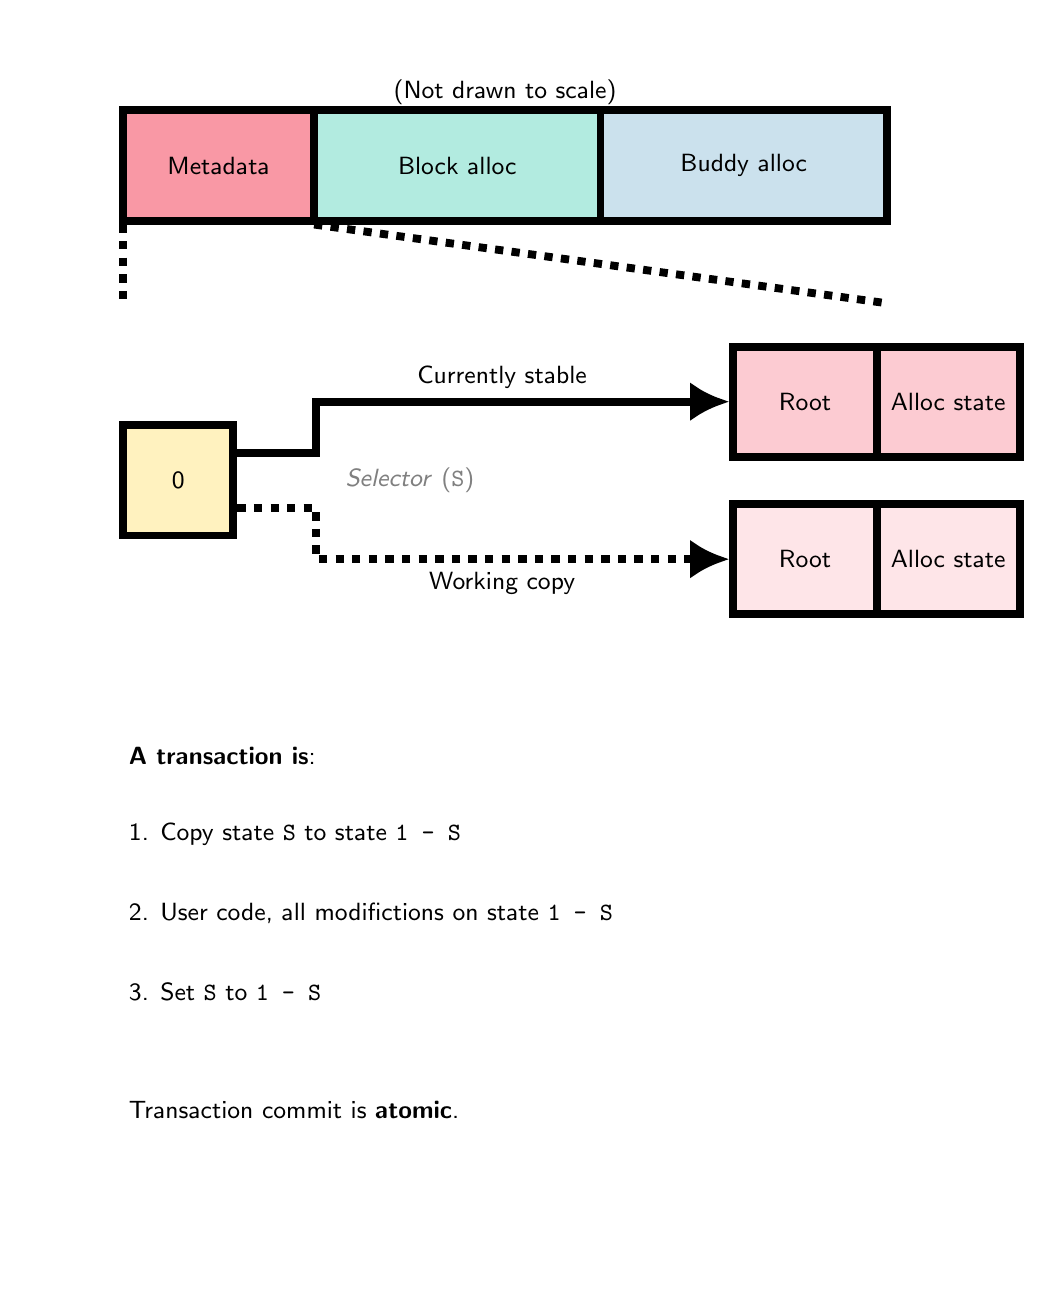
\begin{tikzpicture}
        \path (0, 0) -- (\linewidth, -16);
        \definecolor{mylightblue}{RGB}{151,196,220}
        \definecolor{mylightgreen}{RGB}{102,216,193}
        \definecolor{mylightred}{RGB}{249,152,165}
        \definecolor{mylightyellow}{RGB}{255,230,127}       

        \node[draw, rectangle, line width = 1mm, minimum width = 0.8\linewidth, minimum height = 1.4cm, anchor = north] at (0.5\linewidth, -1) (mem) {};
        \node[align = center, anchor = south] at ([yshift = -1mm] mem.north) {\small (Not drawn to scale)};
        \node[draw, rectangle, line width = 1mm, minimum width = 0.2\linewidth, minimum height = 1.4cm, anchor = west, fill = mylightred] at (mem.west) (meta) {\small Metadata};
        \node[draw, rectangle, line width = 1mm, minimum width = 0.3\linewidth, minimum height = 1.4cm, anchor = west, fill = mylightgreen!50!white] at ([xshift=-\pgflinewidth]meta.east) (alloc1) {\small Block alloc};
        \node[draw, rectangle, line width = 1mm, minimum width = 0.3\linewidth, minimum height = 1.4cm, anchor = west, fill = mylightblue!50!white] at ([xshift=-\pgflinewidth]alloc1.east) (alloc2) {\small Buddy alloc};

        
        \node[draw, rectangle, line width = 1mm, minimum width = 1.4cm, minimum height = 1.4cm, fill = mylightyellow!50!white, anchor = west] at ([yshift = -4cm] mem.west) (sel0) {\small 0};
        %\node[align = center, anchor = south] at ([yshift = 1mm] sel0.north) {\small Selector};

        \node[draw, rectangle, line width = 1mm, minimum width = 0.15\linewidth, minimum height = 1.4cm, anchor = west, fill = mylightred!50!white] at ([xshift = 7cm, yshift = 1cm] sel0.center) (r0) {\small Root};
        \node[draw, rectangle, line width = 1mm, minimum width = 0.15\linewidth, minimum height = 1.4cm, anchor = west, fill = mylightred!50!white] at ([xshift = -\pgflinewidth] r0.east) (r0a) {\small Alloc state};

        \node[draw, rectangle, line width = 1mm, minimum width = 0.15\linewidth, minimum height = 1.4cm, anchor = west, fill = mylightred!25!white] at ([xshift = 7cm, yshift = -1cm] sel0.center) (r1) {\small Root};
        \node[draw, rectangle, line width = 1mm, minimum width = 0.15\linewidth, minimum height = 1.4cm, anchor = west, fill = mylightred!25!white] at ([xshift = -\pgflinewidth] r1.east) {\small Alloc state};

        \path[draw, -{Latex[length = 5mm, width = 5mm]}, line width = 1mm] ([yshift = 3.5mm] sel0.east) -| ([yshift = 1cm, xshift=1cm] sel0.east) -- (r0.west) node [above, pos = 0.45, align = center] {\small Currently stable};
        \path[draw, -{Latex[length = 5mm, width = 5mm]}, line width = 1mm, dashed] ([yshift = -3.5mm] sel0.east) -| ([yshift = -1cm, xshift=1cm] sel0.east) -- (r1.west) node [below, pos = 0.45, align = center] {\small Working copy};
        \node[align = left, anchor = west, text = black!50!white] at ([xshift = 2.75cm] sel0.west) {\small \textit{Selector} (\texttt{S})};

        \path[draw, dashed, line width = 1mm] ([xshift = 0.5\pgflinewidth]meta.south west) -- ([yshift = -1cm, xshift = 0.5\pgflinewidth] meta.south west);
        \path[draw, dashed, line width = 1mm] ([xshift = -0.5\pgflinewidth]meta.south east) -- ([yshift = -1cm, xshift = -0.5\pgflinewidth] alloc2.south east);

        \node[anchor = west, align = left] at ([yshift = -3.5cm] sel0.west) (t0) {\small \textbf{A transaction is}:};
        \node[anchor = west, align = left] at ([yshift = -1cm] t0.west) (t1) {\small 1. Copy state \texttt{S} to state \texttt{1 - S}};
        \node[anchor = west, align = left] at ([yshift = -2cm] t0.west) (t2) {\small 2. User code, all modifictions on state \texttt{1 - S}};
        \node[anchor = west, align = left] at ([yshift = -3cm] t0.west) (t3) {\small 3. Set \texttt{S} to \texttt{1 - S}};
        \node[anchor = west, align = left] at ([yshift = -4.5cm] t0.west) (t4) {\small Transaction commit is \textbf{atomic}.};
        
        
        
      \end{tikzpicture}
    \end{minipage}
    \hfill
    \begin{minipage}{0.48\linewidth}
      \centering \textbf{Persistent types}
      \begin{tikzpicture}
        \path (0, 0) -- (\linewidth, -16);
        
        \node[align = center] at (0, -1.5)                (pbox) {\texttt{PBox<T>}};
        \node[align = center] at ([yshift = -1cm] pbox) (pboxsub) {\small Stores one \texttt{T}};

        \node[draw, rectangle, line width = 1mm, minimum width = 15mm, minimum height = 15mm] at ([yshift = -3cm, xshift = -1.5cm] pbox) (pbox1) {};
        \node[align = center, anchor = north] at ([yshift = -0.1em] pbox1.south) {\small PBox};
        \AllocBlock{[yshift = -3cm, xshift = 1.5cm] pbox}{a1}{$B_1$};
        \node[draw, fill = black, fill opacity = 0.3, minimum width = 20mm, minimum height = 20mm] at (a1.center) {};
        \path[draw, -{Latex[length = 5mm, width = 5mm]}, line width = 1mm] (pbox1.center) -- (a1.west);
        \path[draw, -{Latex[length = 5mm, width = 5mm]}, line width = 1mm, dashed, orange] (a1t.center) -- ([yshift = -1.5cm]a1t.center);
        \path[draw, -{Latex[length = 5mm, width = 5mm]}, line width = 1mm, dashed, cyan] (a1b.center) -- ([yshift = -1.5cm]a1b.center);

        \path[draw, dashed, line width = 1mm] ([xshift = 1.1cm, yshift = 3cm] a1.east) -- ([xshift = 1.1cm, yshift = -3cm] a1.east);
        
        \node at ([xshift = 7cm] pbox) (pboxafter) {};
        \node[draw, rectangle, line width = 1mm, minimum width = 15mm, minimum height = 15mm] at ([yshift = -3cm, xshift = -1.5cm] pboxafter) (pbox2) {};
        \node[align = center, anchor = north] at ([yshift = -0.1em] pbox2.south) {\small PBox};
        \AllocBlock{[yshift = 0cm, xshift = 2.5cm] pboxafter}{a2}{$B_1$};
        \AllocBlock{[yshift = -4.5cm, xshift = 2.5cm] pboxafter}{a3}{$B_2$};
        \node[draw, fill = black, fill opacity = 0.3, minimum width = 20mm, minimum height = 20mm] at (a3.center) {};
        \path[draw, -{Latex[length = 5mm, width = 5mm]}, line width = 1mm] (pbox2.center) -| ([xshift = -1cm] a3.west) -- (a3.west);
        \path[draw, -{Latex[length = 5mm, width = 5mm]}, line width = 1mm, orange] (a2t.center) -- ([xshift = -5mm] a3.north);
        \path[draw, -{Latex[length = 5mm, width = 5mm]}, line width = 1mm, cyan] (a2b.center) -- ([xshift = 5mm] a3.north);
        \path[draw, -{Latex[length = 5mm, width = 5mm]}, line width = 1mm, dashed, orange] (a3t.center) -- ([yshift = -1.5cm]a3t.center);
        \path[draw, -{Latex[length = 5mm, width = 5mm]}, line width = 1mm, dashed, cyan] (a3b.center) -- ([yshift = -1.5cm]a3b.center);
        \node[align = left, text width = 5cm] at ([xshift = 8cm] pbox2.center) {\baselineskip=1pt\small \texttt{deref\_mut}: realloc if first time in transaction\par};

        \node[align = center] at ([yshift = -8cm] pbox) (pvec) {\texttt{PVec<T>}};
        \node[align = center] at ([yshift = -1cm] pvec) (pvecsub) {\small Stores many \texttt{T}};
        \node[draw, rectangle, line width = 1mm, minimum height = 20mm, anchor = west] at ([yshift = -2cm] pvecsub.west) (pvec0) {\small \texttt{len=5}};
        \node[draw, rectangle, line width = 1mm, minimum height = 20mm, anchor = west] at ([xshift = -\pgflinewidth] pvec0.east) (pvec0p) {};
        \path (pvec0.south west) -- (pvec0p.south east) node[below, midway, align = center] {\small PVec};

        \node[draw, rectangle, line width = 1mm, minimum width = 80mm, minimum height = 20mm, anchor = west] at ([xshift = 3cm] pvec0.east) (a4) {};
        \node[draw, rectangle, line width = 1mm, minimum width = 10mm, minimum height = 10mm, anchor = north west] at ([xshift = -\pgflinewidth] a4.north east) (a4t) {}; 
        \node[draw, rectangle, line width = 1mm, minimum width = 10mm, minimum height = 10mm, anchor = south west] at ([xshift = -\pgflinewidth] a4.south east) (a4b) {};
        \path[draw, -{Latex[length = 5mm, width = 5mm]}, line width = 1mm] (pvec0p.center) -- (a4.west);
        \path[draw, -{Latex[length = 5mm, width = 5mm]}, line width = 1mm, dashed, cyan] (a4t.center) -- ([xshift = 1.5cm]a4t.center);
        \path[draw, -{Latex[length = 5mm, width = 5mm]}, line width = 1mm, dashed, orange] (a4b.center) -- ([xshift = 1.5cm]a4b.center);
        \node[minimum width = 25mm, minimum height = 20mm, anchor = west, fill = black, fill opacity = 0.3, line width = 0] at ([xshift = \pgflinewidth] a4.west) (a4fill) {};
        \node[minimum width = 55mm, minimum height = 20mm, anchor = west, fill = black, opacity = 0.3, pattern = {Lines[angle=-45, distance = 6mm, line width = 3mm]}] at ([xshift=-1.5mm] a4fill.east) (a4fill2) {};
        \node[circle, align = center, anchor = center, fill = white, minimum width = 15mm] at (a4.center) {};
        \node[align = center, anchor = center] at (a4.center) {$B_1$};

        \path[draw, decorate, decoration = {brace, amplitude = 10pt, mirror}, black, line width = 1mm] ([yshift = -0.4cm] a4fill.south west) -- ([yshift = -0.4cm, xshift = -1mm] a4fill.south east) node[midway, below, align = center, yshift = -3mm] {\small Items};
        \path[draw, decorate, decoration = {brace, amplitude = 10pt, mirror}, black, line width = 1mm] ([yshift = -0.25cm, xshift = 2mm] a4fill2.south west) -- ([yshift = -0.25cm] a4fill2.south east) node[midway, below, align = center, yshift = -3mm, text width = 5cm] {\baselineskip=1pt\small Allocated but unused\par};
        
      \end{tikzpicture}

    \end{minipage}
  }
  \block{Using a special ``hitchhiker'' tree to implement interior mutability}{
    \newcommand\AllocBlock[3]{
      \node[draw, rectangle, line width = 1mm, minimum width = 16mm, minimum height = 16mm] at (#1) (#2) {#3};
      \node[draw, rectangle, line width = 1mm, minimum width =  8mm, minimum height =  8mm, anchor = north west] at ([xshift = -\pgflinewidth] #2.north east) (#2t) { };
      \node[draw, rectangle, line width = 1mm, minimum width =  8mm, minimum height =  8mm, anchor = south west] at ([xshift = -\pgflinewidth] #2.south east) (#2b) { };
    }

    \begin{tikzpicture}
      \definecolor{mylightblue}{RGB}{151,196,220}
      \definecolor{mylightgreen}{RGB}{102,216,193}
      \definecolor{mylightred}{RGB}{249,152,165}
      \definecolor{mylightyellow}{RGB}{255,230,127}       

      
      \node[draw, rectangle, minimum width = 1.4cm, minimum height = 1.4cm, line width = 1mm, fill = mylightred!20!white] at (0, 0) (inner0s0) { };
      \node[draw, rectangle, minimum width = 1.4cm, minimum height = 1.4cm, line width = 1mm, anchor = west, fill = mylightred!50!white] at ([xshift = -\pgflinewidth] inner0s0.east) (inner0s1) {\small $\infty$};
      \node[draw, rectangle, minimum width = 1.4cm, minimum height = 1.4cm, line width = 1mm, anchor = west, fill = mylightred!50!white] at ([xshift = -\pgflinewidth] inner0s1.east) (inner0s2) {\small 4};
      \node[draw, rectangle, minimum width = 2.8cm, minimum height = 1.4cm, line width = 1mm, anchor = west, fill = orange!30!white] at ([xshift = -\pgflinewidth] inner0s2.east) (inner0b) {\small (8, H)};
      
      \path[draw, decorate, decoration = {brace, amplitude = 10pt}, black, line width = 0.75mm] ([yshift = 2mm] inner0s0.north west) -- ([yshift = 2mm] inner0s2.north east) node[midway, above, yshift = 2mm] {\small Lookup keys};
      \path[draw, decorate, decoration = {brace, amplitude = 10pt}, black, line width = 0.75mm] ([xshift = 2mm] inner0b.north east) -- ([xshift = 2mm] inner0b.south east) node[midway, anchor = west, align = left, xshift = 2mm] {\small Buffer};

      
      \node[draw, rectangle, minimum width = 1.4cm, minimum height = 1.4cm, line width = 1mm, fill = mylightred] at (8, -4) (leaf0k0) {\small 3};
      \node[draw, rectangle, minimum width = 1.4cm, minimum height = 1.4cm, line width = 1mm, anchor = west, fill = mylightred] at ([xshift = -\pgflinewidth] leaf0k0.east) (leaf0k1) {\small 2};
      \node[draw, rectangle, minimum width = 1.4cm, minimum height = 1.4cm, line width = 1mm, anchor = west, fill = mylightred] at ([xshift = -\pgflinewidth] leaf0k1.east) (leaf0k2) {\small 1};
      \node[draw, rectangle, minimum width = 1.4cm, minimum height = 1.4cm, line width = 1mm, anchor = north, fill = mylightgreen] at ([yshift = \pgflinewidth] leaf0k0.south) (leaf0v0) {\small C};
      \node[draw, rectangle, minimum width = 1.4cm, minimum height = 1.4cm, line width = 1mm, anchor = north, fill = mylightgreen] at ([yshift = \pgflinewidth] leaf0k1.south) (leaf0v1) {\small B};
      \node[draw, rectangle, minimum width = 1.4cm, minimum height = 1.4cm, line width = 1mm, anchor = north, fill = mylightgreen] at ([yshift = \pgflinewidth] leaf0k2.south) (leaf0v2) {\small A};

      \path[draw, decorate, decoration = {brace, amplitude = 10pt}, black, line width = 0.75mm] ([xshift = 2mm] leaf0k2.north east) -- ([xshift = 2mm, yshift = 2mm] leaf0k2.south east) node[midway, anchor = west, align = left, xshift = 2mm] {\small Keys};
      \path[draw, decorate, decoration = {brace, amplitude = 10pt}, black, line width = 0.75mm] ([xshift = 2mm, yshift = -2mm] leaf0v2.north east) -- ([xshift = 2mm] leaf0v2.south east) node[midway, anchor = west, align = left, xshift = 2mm] {\small Values};


      \node[draw, rectangle, minimum width = 1.4cm, minimum height = 1.4cm, line width = 1mm, fill = mylightred!20!white] at (0, -4) (leaf1k0) {};
      \node[draw, rectangle, minimum width = 1.4cm, minimum height = 1.4cm, line width = 1mm, anchor = west, fill = mylightred] at ([xshift = -\pgflinewidth] leaf1k0.east) (leaf1k1) {\small 7};
      \node[draw, rectangle, minimum width = 1.4cm, minimum height = 1.4cm, line width = 1mm, anchor = west, fill = mylightred] at ([xshift = -\pgflinewidth] leaf1k1.east) (leaf1k2) {\small 6};
      \node[draw, rectangle, minimum width = 1.4cm, minimum height = 1.4cm, line width = 1mm, anchor = north, fill = mylightgreen!20!white] at ([yshift = \pgflinewidth] leaf1k0.south) (leaf1v0) {};
      \node[draw, rectangle, minimum width = 1.4cm, minimum height = 1.4cm, line width = 1mm, anchor = north, fill = mylightgreen] at ([yshift = \pgflinewidth] leaf1k1.south) (leaf1v1) {\small G};
      \node[draw, rectangle, minimum width = 1.4cm, minimum height = 1.4cm, line width = 1mm, anchor = north, fill = mylightgreen] at ([yshift = \pgflinewidth] leaf1k2.south) (leaf1v2) {\small F};
      
      \path[draw, -{Latex[length = 5mm, width = 5mm]}, line width = 1mm] (inner0s2.south) |- ([yshift = 1.5cm] leaf0k1.north) -- (leaf0k1.north);
      \path[draw, -{Latex[length = 5mm, width = 5mm]}, line width = 1mm] (inner0s1.south) -- (leaf1k1.north);

      \node[align = right, anchor = east] at (inner0s0.west) {\small Inner node};
      \node[align = right, anchor = east] at (leaf1k0.south west) {\small Leaf node};

      \node[align = left, anchor = north west] at (15, 1.8) (algo0) {\small \textbf{Inserting a (k, p) pair in a tree node}:};
      \node[align = left, anchor = north west] at ([xshift = 1cm, yshift = 5mm] algo0.south west) (algo1) {\small If leaf: \textbf{insert} inside, promote to inner if full.};
      \node[align = left, anchor = north west] at ([yshift = 4mm] algo1.south west) (algo2) {\small If inner:};
      \node[align = left, anchor = north west] at ([xshift = 1cm, yshift = 3mm] algo2.south west) (algo3) {\small If the buffer is full:};
      \node[align = left, anchor = north west, text width = 14cm] at ([xshift = 1cm, yshift = 3mm] algo3.south west) (algo4) {\baselineskip=1pt\small \textbf{Flush the buffer} into the children, eventually promoting self to an upper node.\par};
      \node[align = left, anchor = north west, text width = 14cm] at ([xshift = -1cm, yshift = 3mm] algo4.south west) (algo5) {\baselineskip=1pt\small \textbf{Insert} in the buffer\par};

      \path[draw, line width = 0.5mm] ([xshift = -0.2cm, yshift = -2mm] algo1.north west) -- ([xshift = -1.2cm, yshift = 2mm] algo5.south west);
      \path[draw, line width = 0.5mm] ([xshift = -0.2cm, yshift = -2mm] algo3.north west) -- ([xshift = -0.2cm, yshift = 2mm] algo5.south west);
      \path[draw, line width = 0.5mm] ([xshift = -0.2cm, yshift = -2mm] algo4.north west) -- ([xshift = -0.2cm, yshift = 2mm] algo4.south west);

      \node[draw, circle, fill = black, minimum size = 4mm, inner sep = 0pt] at (-4, -10) (t0) {};
      \node[draw, circle, fill = black, minimum size = 4mm, inner sep = 0pt] at ([xshift = 1cm, yshift =  1cm] t0.center) (t1) {};
      \node[draw, circle, fill = black, minimum size = 4mm, inner sep = 0pt] at ([xshift = 1cm, yshift =  0cm] t0.center) (t2) {};
      \node[draw, circle, fill = black, minimum size = 4mm, inner sep = 0pt] at ([xshift = 1cm, yshift = -1cm] t0.center) (t3) {};
      \node[draw, circle, fill = black, minimum size = 4mm, inner sep = 0pt] at ([xshift = 1cm, yshift =  0.5cm] t1.center) (t4) {};
      \node[draw, circle, fill = black, minimum size = 4mm, inner sep = 0pt] at ([xshift = 1cm, yshift = -0.5cm] t1.center) (t5) {};
      \node[draw, circle, fill = black, minimum size = 4mm, inner sep = 0pt] at ([xshift = 2cm, yshift =  0cm] t2.center) (t6) {};
      \node[draw, circle, fill = black, minimum size = 4mm, inner sep = 0pt] at ([xshift = 1cm, yshift =  0cm] t4.center) (t7) {};

      \path[draw, line width = 0.75mm] (t0.center) -- (t1.center);
      \path[draw, line width = 0.75mm] (t0.center) -- (t2.center);
      \path[draw, line width = 0.75mm] (t0.center) -- (t3.center);
      \path[draw, line width = 0.75mm] (t1.center) -- (t4.center);
      \path[draw, line width = 0.75mm] (t1.center) -- (t5.center);
      \path[draw, line width = 0.75mm] (t2.center) -- (t6.center);
      \path[draw, line width = 0.75mm] (t4.center) -- (t7.center);

      \node[anchor = north west, align = left, text width = 30cm] at ([xshift = 1cm, yshift = 0.75em] t7.center) {Persistent data structures are \textbf{arborescent} (tree-like). This is at odds with Rust's interior mutability (\texttt{Cell}, \dots) in a persistent context (can't trace mutations up to the root).};


      \node[draw, rectangle, line width = 1mm, minimum size = 20mm] at (-2, -15) (cell) {\small43};
      \node[align = center, anchor = south] at (cell.north) {\small \texttt{Cell}};

      \path[draw, line width = 1mm, -{Latex[width = 5mm, length = 5mm]}] ([yshift = -1cm]cell.south) -- (cell.south) node[pos = 0, anchor = north] {\small Call to \texttt{borrow\_mut}};

      \node[draw, rectangle, inner sep = 0, minimum size = 20mm, line width = 1.5mm, anchor = west, fill = mylightred!20!white] at ([xshift = 10cm] cell.east) (x0l0) {};
      \node[draw, rectangle, inner sep = 0, minimum size = 20mm, line width = 1.5mm, anchor = west, fill = mylightred!50!white] at ([xshift = -\pgflinewidth] x0l0.east) (x0l1) {};
      \node[draw, rectangle, inner sep = 0, minimum size = 20mm, line width = 1.5mm, anchor = west, fill = mylightred!50!white] at ([xshift = -\pgflinewidth] x0l1.east) (x0l2) {};
      \node[draw, rectangle, inner sep = 0, minimum size = 20mm, line width = 1.5mm, anchor = west, fill = orange!30!white] at ([xshift = -\pgflinewidth] x0l2.east) (x0b) {};

      \node[draw, rectangle, inner sep = 0, minimum size = 20mm, line width = 1mm, anchor = west, fill = mylightred!50!white] at ([xshift = -9cm, yshift = -3cm] x0l1.south east) (x1l0) {};
      \node[draw, rectangle, inner sep = 0, minimum size = 20mm, line width = 1mm, anchor = west, fill = mylightred!50!white] at ([xshift = -\pgflinewidth] x1l0.east) (x1l1) {};
      \node[draw, rectangle, inner sep = 0, minimum size = 20mm, line width = 1mm, anchor = west, fill = mylightred!50!white] at ([xshift = -\pgflinewidth] x1l1.east) (x1l2) {};
      \node[draw, rectangle, inner sep = 0, minimum size = 20mm, line width = 1mm, anchor = west, fill = orange!30!white] at ([xshift = -\pgflinewidth] x1l2.east) (x1b) {};

      \node[draw, rectangle, inner sep = 0, minimum size = 20mm, line width = 1.5mm, anchor = west, fill = mylightred!50!white] at ([xshift = 3cm, yshift = -3cm] x0l1.south east) (x2l0) {};
      \node[draw, rectangle, inner sep = 0, minimum size = 20mm, line width = 1.5mm, anchor = west, fill = mylightred!50!white] at ([xshift = -\pgflinewidth] x2l0.east) (x2l1) {};
      \node[draw, rectangle, inner sep = 0, minimum size = 20mm, line width = 1.5mm, anchor = west, fill = mylightred!50!white] at ([xshift = -\pgflinewidth] x2l1.east) (x2l2) {};
      \node[draw, rectangle, inner sep = 0, minimum size = 20mm, line width = 1.5mm, anchor = west, fill = orange!30!white] at ([xshift = -\pgflinewidth] x2l2.east) (x2b) {};

      \node[draw, rectangle, inner sep = 0, minimum size = 20mm, line width = 1.5mm, anchor = west, fill = mylightred!30!white] at ([yshift = -3cm, xshift = 10mm] x2l0.south west) (x3l0) {};
      \node[draw, rectangle, inner sep = 0, minimum size = 20mm, line width = 1.5mm, anchor = west, fill = mylightred!30!white] at ([xshift = -\pgflinewidth] x3l0.east) (x3l1) {};
      \node[draw, rectangle, inner sep = 0, minimum size = 20mm, line width = 1.5mm, anchor = west, fill = mylightred] at ([xshift = -\pgflinewidth] x3l1.east) (x3l2) {\small \textbf{43}};
      \node[draw, rectangle, inner sep = 0, minimum size = 20mm, line width = 1.5mm, anchor = north west, fill = mylightgreen!30!white] at ([yshift =  \pgflinewidth] x3l0.south west) (x3v0) {};
      \node[draw, rectangle, inner sep = 0, minimum size = 20mm, line width = 1.5mm, anchor = west, fill = mylightgreen!30!white] at ([xshift = -\pgflinewidth] x3v0.east) (x3v1) {};
      \node[draw, rectangle, inner sep = 0, minimum size = 20mm, line width = 1.5mm, anchor = west, fill = mylightgreen] at ([xshift = -\pgflinewidth] x3v1.east) (x3v2) {};
      
      \path[draw, -{Latex[width = 5mm, length = 5mm]}, line width = 0.75mm] (x0l1.center) |- ([yshift = 1cm] x1l1.north east) -- (x1l1.north east);
      \path[draw, -{Latex[width = 5mm, length = 5mm]}, line width = 1.25mm] (x0l2.center) |- ([yshift = 1cm] x2l1.north east) -- (x2l1.north east);
      \path[draw, -{Latex[width = 5mm, length = 5mm]}, line width = 0.75mm, dashed] (x1l0.center) -- ([yshift = -1cm] x1l0.south);
      \path[draw, -{Latex[width = 5mm, length = 5mm]}, line width = 0.75mm, dashed] (x1l1.center) -- ([yshift = -1cm] x1l1.south);
      \path[draw, -{Latex[width = 5mm, length = 5mm]}, line width = 0.75mm, dashed] (x1l2.center) -- ([yshift = -1cm] x1l2.south);

      \path[draw, -{Latex[width = 5mm, length = 5mm]}, line width = 0.75mm, dashed] (x2l0.center) -- ([yshift = -1cm] x2l0.south);
      \path[draw, -{Latex[width = 5mm, length = 5mm]}, line width = 0.75mm, dashed] (x2l1.center) -- ([yshift = -1cm] x2l1.south);

      \path[draw, -{Latex[width = 5mm, length = 5mm]}, line width = 1.25mm] (x2l2.center) |- ([yshift = 1cm] x3l1.north) -- (x3l1.north);

      \node[align = left, anchor = west, text width = 14cm] at ([xshift = 3cm] x0b.east) {\small The path in \textbf{bold} is copied-on-write before allowing modification.\par};

      \path[draw, -{Latex[width = 5mm, length = 5mm]}, line width = 1mm] (cell.east) -- (x0l0.west) node[midway, above] {\small Lookup in pool metadata} node[midway, below] {\small cell tree.};

      \AllocBlock{[yshift = -10cm, xshift = 4cm] cell.south}{alloc0}{$B_7$};
      \AllocBlock{[xshift = 4cm] alloc0.center}{alloc1}{$B_8$};
      \path[draw, -{Latex[length = 5mm, width = 5mm]}, line width = 1mm, dashed, cyan]   ([xshift = -2cm, yshift =  4mm] alloc0.center) -- ([yshift =  4mm] alloc0.west);
      \path[draw, -{Latex[length = 5mm, width = 5mm]}, line width = 1mm, dashed, orange] ([xshift = -2cm, yshift = -4mm] alloc0.center) -- ([yshift = -4mm] alloc0.west);

      \path[draw, -{Latex[length = 5mm, width = 5mm]}, line width = 1mm, cyan]   (alloc0t.center) -- ([yshift =  4mm] alloc1.west);
      \path[draw, -{Latex[length = 5mm, width = 5mm]}, line width = 1mm, orange] (alloc0b.center) -- ([yshift = -4mm] alloc1.west);

      \path[draw, -{Latex[length = 5mm, width = 5mm]}, line width = 1mm, dashed, cyan]   (alloc1t.center) -- ([xshift = 1cm] alloc1t.east);
      \path[draw, -{Latex[length = 5mm, width = 5mm]}, line width = 1mm, dashed, orange] (alloc1b.center) -- ([xshift = 1cm] alloc1b.east);

      \path[draw, -{Latex[length = 5mm, width = 5mm]}, line width = 1mm, dashed] ([xshift = -5mm] x3v2.south) |- ([xshift = -85mm, yshift = -6mm] x3v2.south) |- ([yshift = 1cm] alloc0.north) -- (alloc0.north) node [pos = 0, above, align = left, anchor = south west, xshift = 1.7cm] {\small Previous allocated block}; 
      \path[draw, -{Latex[length = 5mm, width = 5mm]}, line width = 1mm] ([xshift = 5mm] x3v2.south) |- ([yshift = -1cm, xshift = 4mm] alloc1.south) -- ([xshift = 4mm] alloc1.south) node [pos = 0, below, align = left, anchor = north west, xshift = 4.7cm] {\small Newly allocated block};

      \path[draw, -{Latex[length = 5mm, width = 5mm]}, line width = 1mm] ([xshift = -4mm] alloc1.south) |- ([yshift = -11.85cm] cell.south) -- ([yshift = -4cm] cell.south) node [pos = 1, anchor = south] {\small Returned reference.};
      
    \end{tikzpicture}
  }
  
\end{columns}
\end{document}
